
%%%%%%%%%%%%%%%%%%%%%%%%%%%%%%%%%%%%%%%%%%%%%%%%%%
\begin{frame}{\Huge Objective of presentation}

\vskip -0.5cm

Explain how

\vskip 0.6cm

\begin{center}
\textbf{\LARGE H\'{a}jek's SRSWOR Central Limit Theorem}
\end{center}

\vskip 0.1cm

is a real clever application of

\vskip 0.3cm

\begin{itemize}
\item	\textbf{\LARGE a ``classical'' Central Limit Theorem}
		\vskip 0.05cm
		{\small(the Lindeberg Central Limit Theorem)}
		\vskip 0.6cm
\item	\textbf{\LARGE Slutsky's Theorems}
		\vskip 0.05cm
		{\small(useful tool from mathematical statistics)}
\end{itemize}

\end{frame}
\normalsize

%%%%%%%%%%%%%%%%%%%%%%%%%%%%%%%%%%%%%%%%%%%%%%%%%%
\begin{frame}{\LARGE Why care about Central Limit Theorems?}

\begin{center}
\textbf{\Huge
Confidence Intervals
\vskip 1.0cm
Margin of Error
\vskip 1.0cm
Hypothesis Testing
}
\end{center}

\end{frame}
\normalsize

%%%%%%%%%%%%%%%%%%%%%%%%%%%%%%%%%%%%%%%%%%%%%%%%%%
\begin{frame}{\LARGE H\'{a}jek's SRSWOR Central Limit Theorem}

\vskip -0.1cm

{\large Roughly,

\vskip 0.2cm
\small
$U$ \;$:=$\; a finite population.
\quad
$N$ \;$:=$\; size of $U$.

$\left\{\;y_{i}\;\right\}_{i \in U}$ \;$=$\; population characteristic.

$n$ \;$:=$\; SRSWOR sample size.
\quad
{\color{red}$s$} \;$=$\; SRSWOR sample of size $n$.

\vskip 0.2cm
\large
\begin{center}
The ``centred standardized'' SRSWOR sample mean
\begin{equation*}
	Z_{n}({\color{red}s}) :=
	\left.\left(\dfrac{1}{n}\,\underset{i\,\in\,{\color{red}s}}{\sum}\,(y_{i}\;-\;\overline{y}_{U})\right)\right\slash
	{\color{faintblue}
	\underset
		{\sqrt{\left(1 - \frac{n}{N}\right)\frac{S^{\,2}_{U}}{n}}}
		{\underbrace{\color{black}\sqrt{\Var(\textnormal{numerator})}}}
	}
\end{equation*}
\vskip -0.2cm
tends to $N(0,1)$ {\color{gcblue}\textbf{in distribution}},\; as \;$n$\,,\;{\color{red}$N\,-n$} \;$\longrightarrow$\; $\infty$
\vskip 0.1cm
provided the {\color{red}``H\'{a}jek condition''} (on the $y_{i}$'s) holds.
\end{center}
}

\end{frame}
\normalsize

%%%%%%%%%%%%%%%%%%%%%%%%%%%%%%%%%%%%%%%%%%%%%%%%%%
\begin{frame}{\Huge Slutsky's Theorems}

\begin{center}
\vskip -0.75cm

\begin{center}

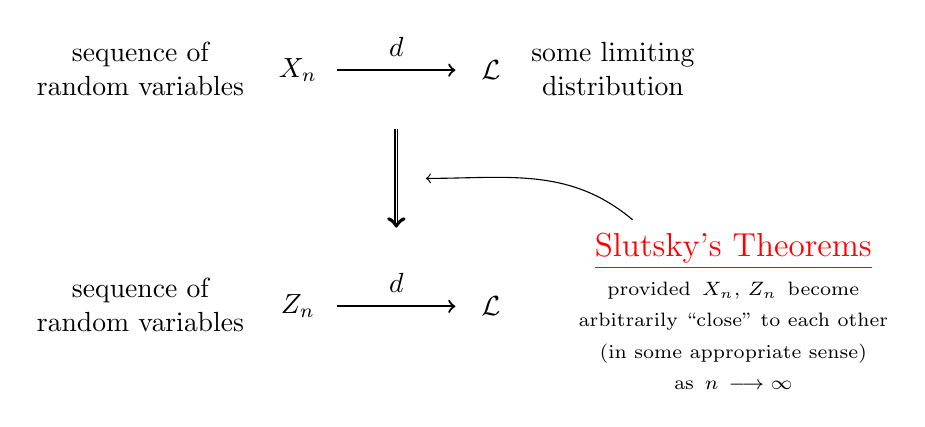
\begin{tikzpicture}

\pause
\node at (2,0) {$Z_{n}$};
\node at (0,0.2) {sequence of};
\node at (0,-0.2) {random variables};
\node at (2,3) {$X_{n}$};
\node at (0,3.2) {sequence of};
\node at (0,2.8) {random variables};

\pause
\node at (3.25,3.3) {$d$};
\draw [->,thick] (2.5,3) -- (4,3);
\node at (4.45,3.0) {$\mathcal{L}$};
\node at (6,3.2) {some limiting};
\node at (6,2.8) {distribution};

\pause
\node at (7.53,0.7) {\large\color{red}\underline{Slutsky's Theorems}};
\draw [->,double] (3.25,2.25) -- (3.25,1.0);
\draw [<-] (3.625,1.625) to [out=0,in=140] (6.25,1.1);
\node at (3.25,0.3) {$d$};
\draw [->,thick] (2.5,0) -- (4,0);
\node at (4.45,0) {$\mathcal{L}$};

\pause
\node at (7.53,0.2) {\scriptsize provided \,$X_{n},\,Z_{n}$\, become};
\node at (7.53,-0.2) {\scriptsize arbitrarily ``close'' to each other};
\node at (7.53,-0.6) {\scriptsize (in some appropriate sense)};
\node at (7.53,-1.0) {\scriptsize as \,$n\,\longrightarrow \infty$};

%%%%%%%%%%%%%
%\pause
%\node at (7.85,0.275) {\scriptsize H\'{a}jek's sampling design};

%\pause
%\node at (7.86,0.0) {\tiny (H\'{a}jek's fundamental inequality)};
%\pause
%\node at (7.53,-0.4) {\scriptsize\color{gcblue}$n\,,\;N-n\,\longrightarrow \infty$};

\onslide<1-> % added to force frame number to be displayed at footline.
\end{tikzpicture}

\end{center}

\end{center}

\end{frame}

%%%%%%%%%%%%%%%%%%%%%%%%%%%%%%%%%%%%%%%%%%%%%%%%%%
\begin{frame}{\LARGE The Most Famous Central Limit Theorem}

$W_{1}$, \;$W_{2}$, \;$\ldots$\; are independent and identically distributed,

with (common) finite expectation value $\mu$ and variance $\sigma^{2}$.

\vskip 0.2cm
Then,
\large
\begin{center}
the ``centred standardized'' sample mean
\begin{equation*}
	X_{n} \;:=\;
	\left.
		\left(\dfrac{1}{n}\,\overset{n}{\underset{i\,=1}{\sum}}\,(W_{i}\;-\;\mu)\right)
	\right\slash\!\!\!\!
	{\color{faintblue}\underset{{\color{white}MMMMMM}\left.\sqrt{n\,\sigma^{2}}\right\slash n \;\,=\;\, \sigma/\sqrt{n}}{\underbrace{\color{black}\sqrt{\Var(\textnormal{numerator})}}}}
\end{equation*}
tends to $N(0,1)$ {\color{gcblue}\textbf{in distribution}},\; as \;$n$ \,$\longrightarrow$\, $\infty$.
\end{center}

\pause
\vskip 0.1cm
{\small\color{red}Not usable to prove H\'{a}jek's SRSWOR CLT, because
\pause
\begin{center}
\vskip -0.2cm
SRSWOR sample mean does NOT have  I.I.D. summands.
\end{center}
}

\end{frame}
\normalsize

%%%%%%%%%%%%%%%%%%%%%%%%%%%%%%%%%%%%%%%%%%%%%%%%%%
\begin{frame}{\huge NOT identically distributed ...}

\pause
\begin{center}
\textit{\Huge No problem!}
\end{center}

\pause
{\LARGE
Use
\begin{center}
\vskip -0.2cm
\textbf{\Huge Lindeberg's
\vskip 0.2cm
Central Limit Theorem}
\end{center}
\vskip 0.2cm
instead.
}

\end{frame}
\normalsize

%%%%%%%%%%%%%%%%%%%%%%%%%%%%%%%%%%%%%%%%%%%%%%%%%%
%\begin{frame}{\LARGE Lindeberg's Central Limit Theorem {\large\color{gcblue}implies}}
%
%$W_{1}$, \;$W_{2}$, \;$\ldots$\; are independent {\color{faintblue}\sout{and identically distributed}},
%
%{\color{faintblue}\sout{with (common) finite expectation value $\mu$ and variance $\sigma^{2}$}}
%
%each having finite expectation value $\mu_{i}$ and finite variance $\sigma_{i}^{2}$.
%
%\vskip 0.2cm
%Then,
%\large
%\begin{center}
%the ``centred standardized'' sample mean
%\begin{equation*}
%	X_{n} \;:=\;
%	\left.\left(\dfrac{1}{n}\,\overset{n}{\underset{i\,=1}{\sum}}\,(W_{i}\;-\;\mu_{i})\right)\right\slash
%	{\color{faintblue}
%		\underset
%			{\left.\sqrt{\sum_{i=1}^{n}\sigma_{i}^{2}}\right\slash n}
%			{\underbrace{\color{black}\sqrt{\Var(\textnormal{numerator})}}}
%	}
%\end{equation*}
%\vskip -0.2cm
%tends to $N(0,1)$ {\color{gcblue}\textbf{in distribution}},\; as \;$n$ \,$\longrightarrow$\, $\infty$,
%\vskip 0.1cm
%provided \pause the {\color{red}Lindeberg condition} (on the $W_{i}$'s) holds.
%\end{center}
%
%\vskip -0.1cm
%{\tiny\color{faintred}
%\begin{equation*}
%\textnormal{Lindeberg's condition:}
%\quad
%\textnormal{For each $\varepsilon > 0$},
%\;
%\lim_{n\rightarrow\infty}\,
%\dfrac{1}{\Sigma^{2}_{n}}
%\sum_{j=1}^{n}\,
%E\!\left[\;
%\left(W_{j} - \mu_{j}\right)^{2}
%\cdot
%I_{\left\{\left\vert W_{j} - \mu_{j}\right\vert \;\geq\; \varepsilon \Sigma_{n}\right\}}
%\;\right]
%\;=\;
%0.
%\end{equation*}
%}
%
%\end{frame}
%\normalsize

%%%%%%%%%%%%%%%%%%%%%%%%%%%%%%%%%%%%%%%%%%%%%%%%%%
\begin{frame}{\LARGE}

{\Huge
\begin{center}
Lindeberg's CLT alone

\vskip 0.2cm
still does NOT imply

\vskip 0.2cm
H\'{a}jek's SRSWOR CLT.

\vskip 0.2cm
{\normalsize\color{red}Summands in SRSWOR sample mean are NOT independent.}
\end{center}
}

\end{frame}
\normalsize

%%%%%%%%%%%%%%%%%%%%%%%%%%%%%%%%%%%%%%%%%%%%%%%%%%
\begin{frame}{\Huge H\'{a}jek's clever solution to tackle non-independence}

\pause
\begin{center}
\textbf{\underline{\LARGE H\'{a}jek Sampling Design}}

\pause
\vskip 0.3cm
{\scriptsize
$U$ \;$:=$\; a finite population.
\;
$N$ \;$:=$\; $\vert\;U\;\vert$.
\;
$\left\{\;y_{i}\;\right\}_{i \in U}$ \;$=$\; population characteristic.

$n \in \{\,1,2,\ldots,N-1\,\}$.
}
\end{center}

\pause
\vskip -0.3cm
Choose \,\textbf{\color{red}two}\, samples $s_{0}$,\, $s_{1}$ \,$\subset U$\, such that:
\begin{itemize}
\pause
\item	$s_{0}$ \;$=$\; SRSWOR of size $n$,
\pause
\item	$s_{1}$ \;$=$\; {\color{red}Bernoulli} sample, with unit selection probability $=$ $n/N$,
\pause
\item	the {\color{red}H\'{a}jek's fundamental inequality} holds:
\pause
		{\scriptsize
		\vskip -0.1cm
		\begin{equation*}
		E\!\left[\;\dfrac{\left(Z_{n}({\color{faintred}s_{0}}) - X_{n}({\color{faintred}s_{1}})\right)^{2}}{\Var\!\left[\,X_{n}\,\right]}\;\right]
		\;\leq\;
		\sqrt{\dfrac{1}{n} + \dfrac{1}{N-n}}
		\end{equation*}
		}
\end{itemize}

\pause
\begin{center}
\vskip 0.0cm
{\small\color{gcblue}H\'{a}jek proved that the above sampling design is feasible.}
\end{center}

\end{frame}

%%%%%%%%%%%%%%%%%%%%%%%%%%%%%%%%%%%%%%%%%%%%%%%%%%
\begin{frame}{\Large Outline of Proof of \LARGE \,H\'{a}jek's \,SRSWOR\, CLT}

\begin{center}
\vskip -0.75cm

\begin{center}

\begin{tikzpicture}

\pause
\node at (3.25,0.3) {\color{faintgray}$d$};
\draw [->,thick,faintgray] (2.5,0) -- (4,0);
\node at (4.75,0) {\color{faintgray}$N(0,1)$};
\node at (2,0) {$Z_{n}$};
\node at (0,0.4) {SRSWOR};
\node at (0,0) {\scriptsize centred standardized};
\node at (0,-0.4) {sample mean};

\pause
\node at(7.85,0.275) {\scriptsize H\'{a}jek's sampling design};
\node at (2,3) {$X_{n}$};
\node at (0,3.4) {Bernoulli};
\node at (0,3) {\scriptsize centred standardized};
\node at (0,2.6) {sample mean};

\pause
\node at (3.25,3.3) {$d$};
\draw [->,thick] (2.5,3) -- (4,3);
\node at (4.75,3) {$N(0,1)$};

\pause
\draw [<-] (3.25,3.7) to [out=90,in=180] (4.75,4.54);
\node at (5.84,4.5) {\scriptsize\color{red}\underline{Lindeberg's CLT}};
\pause
\node at (7.48,4.1) {\scriptsize {\color{gcblue}H\'{a}jek's condition} (\,$\Rightarrow$\, Lindeberg's condition)};
\pause
\node at (6.25,3.7) {\scriptsize independent summands};

\pause
\node at(7.53,0.7) {\scriptsize\color{red}\underline{Slutsky's Theorems}};
\draw [->,double] (3.25,2.25) -- (3.25,1.0);
\draw [<-] (3.625,1.625) to [out=0,in=135] (6.5,1.0);
\node at (3.25,0.3) {$d$};
\draw [->,thick] (2.5,0) -- (4,0);
\node at (4.75,0) {$N(0,1)$};

\pause
%\node at(7.86,0.0) {\tiny (H\'{a}jek's fundamental inequality)};
\node at(8.00,-0.375)
{\tiny
$\left(\!\!\begin{array}{c}
	\textnormal{H\'{a}jek's fundamental inequality} \\
	\rho(Z_{n},X_{n})\leq \sqrt{\dfrac{1}{n} + \dfrac{1}{N-n}}
\end{array}\!\!\right)$
};
\pause
\node at(7.53,-1.0) {\scriptsize\color{gcblue}$n\,,\;N-n\,\longrightarrow \infty$};

\onslide<1-> % added to force frame number to be displayed at footline.
\end{tikzpicture}

\end{center}

\end{center}

\end{frame}

%%%%%%%%%%%%%%%%%%%%%%%%%%%%%%%%%%%%%%%%%%%%%%%%%%
